\documentclass{article}
\usepackage[utf8]{inputenc}
\usepackage{natbib}
\usepackage{graphicx}
\usepackage{vmargin}
\usepackage{hyperref}
\usepackage{booktabs}
\usepackage{multirow}
\usepackage{siunitx}
\setpapersize{A4}
\setlength{\parskip}{\baselineskip}%
\setlength{\parindent}{0pt}%

\title{Entregable WEKA}
\author{Laura Rodríguez Navas \\ rodrigueznavas@posgrado.uimp.es}
\date{Mayo 2020}

\begin{document}
	
	\maketitle
	
	\section*{Preparación de datos}
	
	Consideramos la base de datos \href{https://poliformat.upv.es/portal/site/ESP_0_2718/page/4b26ee25-8292-4b01-ae40-2c81d8a63ebd}{Prostate} definida sobre 12600 variables predictivas (todas numéricas) y una variable clase binaria \{Tumor, Normal\}. Está formada por 136 registros y en ella no existen valores desconocidos. Pero está ordenada en función de la variable clase. Como consecuencia, tenemos que aleatorizar la base de datos. Para ello se aplica un filtro a nivel de registro, concretamente de tipo no supervisado llamado \textit{Ramdomize}. Usando los parámetros por defecto después de aplicar el filtro comprobaremos que la base de datos se ha aleatorizado.
	
	Analizando un poco la base de datos vemos que el número de registros disponibles (136) es bajo en comparación con el número de atributos (12601). Así, vamos a tratar con un problema de alta dimensionalidad y poca muestra.
	
	Para la clasificación se utilizarán los clasificadores Naive Bayes y J48 (C4.5). El clasificador Naive Bayes es muy buen clasificador en problemas con un número elevado de variables predictoras, como en este caso.
	
	\section*{Clasificación}
	
	Primero se usan los clasificadores Naive Bayes y J48 (C4.5) en una validación cruzada de 5 carpetas (5cv) sobre el conjunto inicial de la base de datos, obteniendo así una medida inicial que se intentará mejorar.
	
	Se consideran dos parámetros de rendimiento para la evaluación de los resultados de las clasificaciones. Los parámetros son los registros clasificados correctamente (Accuracy) y los registros no clasificados correctamente (Error Rate). 
	
	Después de realizar la primera clasificación obtenemos los siguientes resultados:
	
	\begin{center}
		\begin{tabular}{ |c|c|c| } 
			\hline
			Clasificador & Acc. en \% & ERR en \% \\
			\hline
			Naive Bayes & 51.1471 & 44.8529 \\ 
			J48 (C4.5) & 80.1471 & 19.8529 \\ 
			\hline
		\end{tabular}
	\end{center}
	
	\newpage
	
	Inicialmente y sin la aplicación de algún tipo mejora, podemos observar que el algoritmo J48 (C4.5) nos da una clasificación aceptable y clasifica mucho mejor en comparación con el algoritmo Naive Bayes. El algoritmo Naive Bayes no hace una buena clasificación. Se puede pensar que se debe a la alta presencia de variables relevantes y redundantes en la base de datos, ya que sabemos que Naive Bayes es un algoritmo muy sensible a este caso.
	
	\section*{Mejoras}
	
	En este apartado se muestran mejoras que se basan en técnicas de discretización, de selección de variables y una combinación de ambas.
	
	\subsection*{Discretización}
	
	Como la variable clase juega un papel importante y los clasificadores que utilizamos pueden ser entrenados de manera muy eficiente con aprendizaje supervisado, vamos a utilizar una técnica de discretización supervisada. Concretamente, probamos un método supervisado a nivel de atributo basado en la entropía, llamado \href{https://link.springer.com/chapter/10.1007/978-3-642-40897-7_11}{MLDP}. Como resultado, los valores de Accuracy y Error Rate después de esta discretización son:
	
	\begin{center}
		\begin{tabular}{cSSSSS}
			\toprule
			\multirow{2}{*}{Clasificador} &
			\multicolumn{2}{c}{Antes Disc.} &
			\multicolumn{2}{c}{Después Disc.} \\
			& {Acc. in \%} & {ERR in \%} & {Acc. in \%} & {ERR in \%} \\
			\midrule
			Naives Bayes & 51.1471 & 44.8529 & 76.4706 & 23.5294 \\
			J48 (C4.5) & 80.1471 & 19.8529 & 86.7647 & 13.2353 \\
			\bottomrule
		\end{tabular}
	\end{center}
	
	Observamos que es una buena discretización para los dos algoritmos. Como nos ha dado un buen resultado, vamos a combinar esta discretización con técnicas de selección de variables del siguiente apartado.
	
	\subsection*{Selección de variables}
	
	Sabemos que la base de datos contiene muchos atributos y que eso crea un problema, así que para una estimación honesta primero tenemos que reducir el número de atributos de la base de datos. Por ejemplo, para quedarnos con los 200 más representativos y la variable clase, vamos a realizar una selección univariada de tipo Ranker (ver Figura \ref*{fig:ranker}).
	
	Hecha la selección de los 200 atributos más representativos de la base de datos, donde el primer atributo más representativo es el 6185 y el último es el 6776, borraremos el resto de los atributos usando un filtro de registro de tipo no supervisado llamado \textit{Remove}. 
	
	Volvemos a clasificar y vemos que mejora mucho la clasificación de los dos algoritmos si la comparamos con la clasificación inicial, y también mejoran después de la discretización. Los resultados se observan en la siguiente tabla:
	
	\begin{center}
		\begin{tabular}{cSSSSS}
			\toprule
			\multirow{2}{*}{Clasificador} &
			\multicolumn{2}{c}{Inicial} &
			\multicolumn{2}{c}{Ranker} \\
			& {Acc. in \%} & {ERR in \%} & {Acc. in \%} & {ERR in \%} \\
			\midrule
			Naives Bayes & 51.1471 & 44.8529 & 90.4412 & 9.5588 \\
			J48 (C4.5) & 80.1471 & 19.8529 & 91.1765 & 8.8235 \\
			\bottomrule
		\end{tabular}
	\end{center}
	
	Concretamente, la mejora de Naive Bayes es muy significativa. Eso nos demuestra que, al reducir el número de atributos, hemos reducido el número de variables relevantes y redundantes de la base de datos; ya que como hemos comentado anteriormente, Naive Bayes es un algoritmo muy sensible en este caso. 
	
	\renewcommand{\figurename}{Figura}
	\begin{figure}[h]
		\centering
		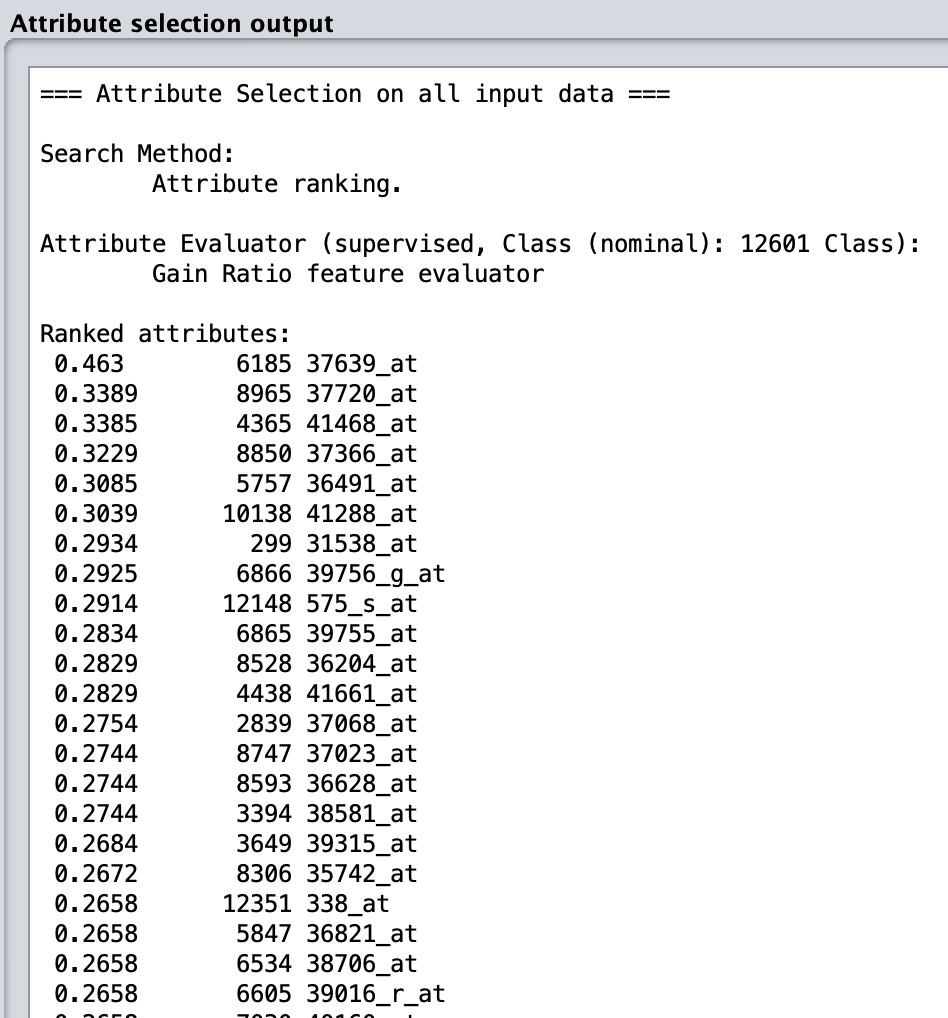
\includegraphics[scale=0.5]{ranker.png}
		\caption{Selección de variables univariada de tipo Ranker.}
		\label{fig:ranker}
	\end{figure}
	
	A continuación, lanzaremos dos selecciones de variables multivariadas de tipo Filter y Wrapper.
	
	Primero, lanzamos la selección de variables multivariada de tipo Filter, que se caracteriza por una técnica de búsqueda CFS (Correlation Feature Subset), y una función de evaluación en selección hacia delante (forward). En este caso la selección de atributos se ve ampliamente reducida a 18 atributos (ver Figura \ref*{fig:filter}).
	
	Después de quedarnos con los 18 atributos más representativos y al volver a clasificar obtenemos:
	
	\begin{center}
		\begin{tabular}{cSSSSS}
			\toprule
			\multirow{2}{*}{Clasificador} &
			\multicolumn{2}{c}{Ranker} &
			\multicolumn{2}{c}{Filter} \\
			& {Acc. in \%} & {ERR in \%} & {Acc. in \%} & {ERR in \%} \\
			\midrule
			Naives Bayes  & 90.4412 & 9.5588 & 95.5882 & 4.4118 \\
			J48 (C4.5) & 91.1765 & 8.8235 & 91.1765 & 8.8235 \\
			\bottomrule
		\end{tabular}
	\end{center}
	
	Otra vez más, el algoritmo Naives Bayes mejora al reducir el número de atributos. En cambio, no hay mejora del algoritmo J48 (C4.5). Podemos decir que el algoritmo J48 (C4.5) no es tan sensible a la reducción de atributos redundantes o irrelevantes, y aunque sigamos reduciendo el número de atributos no habrá mejoras. Lo comprobaremos en la aplicación de la selección multivariada de tipo Wrapper que describimos a continuación.
	
	\newpage
	
	Finalmente, lanzamos una selección multivariada de tipo Wrapper para cada clasificador, con la función de evaluación en selección hacia delante (forward) y obtenemos los resultados:
	
	\begin{center}
		\begin{itemize}
			\item Naive Bayes. La selección de variables se reduce a 5: \{1, 6, 11, 12, 18\}. \\
			\begin{center}
				\begin{tabular}{cSSSSS}
					\toprule
					\multirow{2}{*}{Clasificador} &
					\multicolumn{2}{c}{Filter} &
					\multicolumn{2}{c}{Wrapper} \\
					& {Acc. in \%} & {ERR in \%} & {Acc. in \%} & {ERR in \%} \\
					\midrule
					Naives Bayes & 95.5882 & 4.4118 & 97.7941 & 2.2059 \\
					\bottomrule
				\end{tabular}
			\end{center}
			\item J48 (C4.5). La selección de atributos se reduce a 2: \{4, 6\}. \\
			\begin{center}
				\begin{tabular}{cSSSSS}
					\toprule
					\multirow{2}{*}{Clasificador} &
					\multicolumn{2}{c}{Filter} &
					\multicolumn{2}{c}{Wrapper} \\
					& {Acc. in \%} & {ERR in \%} & {Acc. in \%} & {ERR in \%} \\
					\midrule
					J48 (C4.5) & 91.1765 & 8.8235 & 91.1765 & 8.8235 \\
					\bottomrule
				\end{tabular}
			\end{center}
		\end{itemize} 
	\end{center}
	
	Como conclusión, nos quedamos con la última clasificación ya que es la mejor para los dos algoritmos, los valores de Accuracy son los más altos y los valores de Error Rate los más bajos. Trabajar con variables redundantes o irrelevantes nos puede perjudicar en la capacidad predictiva de nuestro algoritmo. Por ese motivo, algoritmos sensibles a esto, como Naive Bayes, las técnicas de selección de variables producen muchas mejoras en las clasificaciones al reducir el número de este tipo de atributos.
	
	\begin{figure}[h]
		\centering
		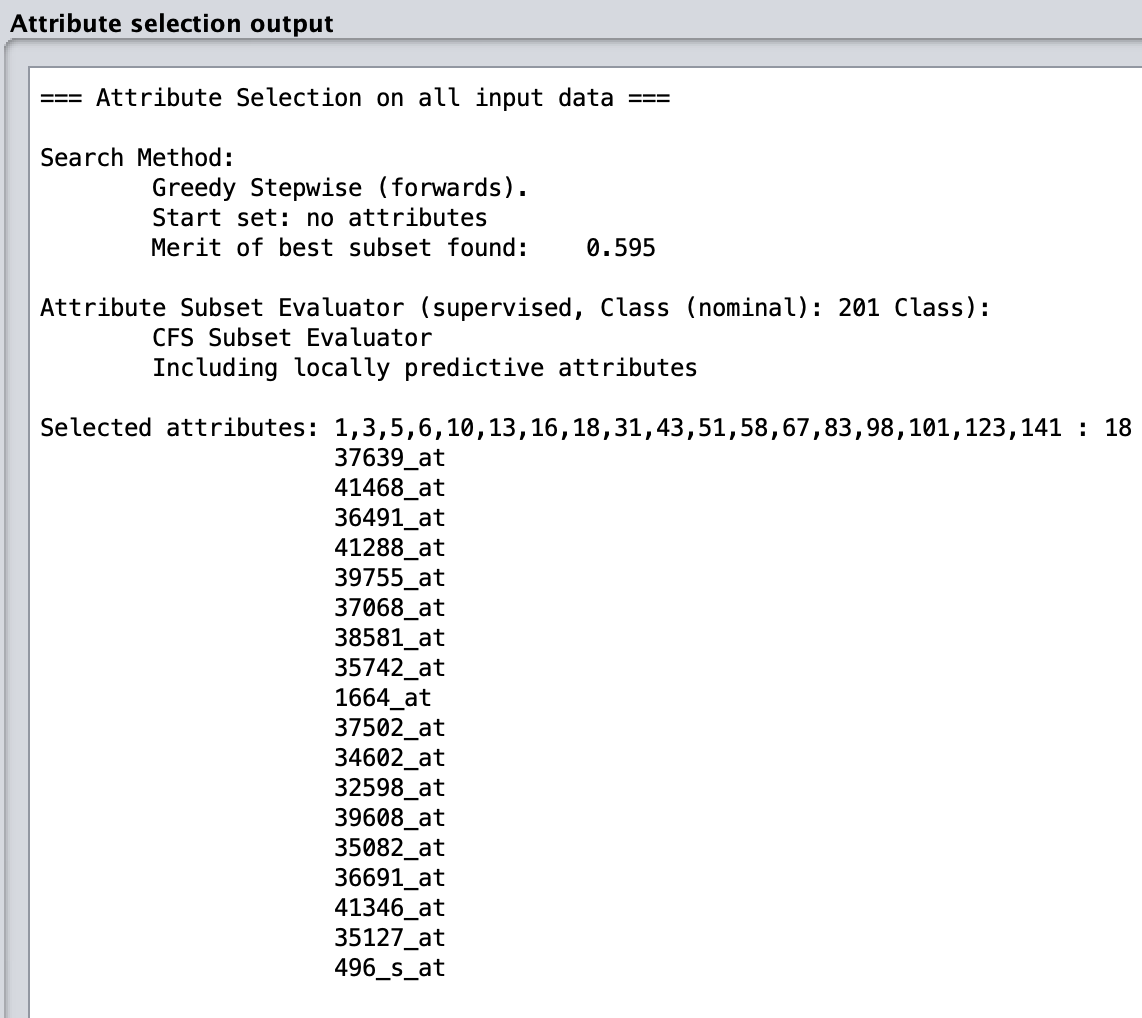
\includegraphics[scale=0.5]{filter.png}
		\caption{Selección de variables multivariada de tipo Filter.}
		\label{fig:filter}
	\end{figure}
	
\end{document}
